\documentclass[12pt]{article}
\usepackage{latexsym,amssymb,amsmath} % for \Box, \mathbb, split, etc.
% \usepackage[]{showkeys} % shows label names
\usepackage{cite} % sorts citation numbers appropriately
\usepackage{path}
\usepackage{url}
\usepackage{verbatim}
\usepackage{graphicx}
\usepackage{array}
\usepackage{multirow}

% horizontal margins: 1.0 + 6.5 + 1.0 = 8.5
\setlength{\oddsidemargin}{0.0in}
\setlength{\textwidth}{6.5in}
% vertical margins: 1.0 + 9.0 + 1.0 = 11.0
\setlength{\topmargin}{0.0in}
\setlength{\headheight}{12pt}
\setlength{\headsep}{13pt}
\setlength{\textheight}{625pt}
\setlength{\footskip}{24pt}

\renewcommand{\textfraction}{0.10}
\renewcommand{\topfraction}{0.85}
\renewcommand{\bottomfraction}{0.85}
\renewcommand{\floatpagefraction}{0.90}
\usepackage{graphicx}
\usepackage{wrapfig}
\usepackage{lscape}
\usepackage{rotating}
\usepackage{epstopdf}
\makeatletter
\setlength{\arraycolsep}{2\p@} % make spaces around "=" in eqnarray smaller
\makeatother

% change equation, table, figure numbers to be counted inside a section:
\numberwithin{equation}{section}
\numberwithin{table}{section}
\numberwithin{figure}{section}

% begin of personal macros
\newcommand{\half}{{\textstyle \frac{1}{2}}}
\newcommand{\eps}{\varepsilon}
\newcommand{\myth}{\vartheta}
\newcommand{\myphi}{\varphi}
\usepackage[utf8]{inputenc}

% Default fixed font does not support bold face
\DeclareFixedFont{\ttb}{T1}{txtt}{bx}{n}{8} % for bold
\DeclareFixedFont{\ttm}{T1}{txtt}{m}{n}{8}  % for normal

% Custom colors
\usepackage{color}
\definecolor{deepblue}{rgb}{0,0,0.5}
\definecolor{deepred}{rgb}{0.6,0,0}
\definecolor{deepgreen}{rgb}{0,0.5,0}
\definecolor{backcolour}{rgb}{0.96,0.96,0.96}

\usepackage{listings}

% cpp style for highlighting
\newcommand\cppstyle{\lstset{
		language=C++,
        basicstyle=\tiny\ttfamily,
		keywordstyle=\color{blue}\ttfamily,
		stringstyle=\color{red}\ttfamily,
		commentstyle=\color{green}\ttfamily,
		morecomment=[l][\color{magenta}]{\#},
		frame=tb,                         % Any extra options here
showstringspaces=false,            % 
backgroundcolor=\color{backcolour}
}}


% cpp environment
\lstnewenvironment{cpp}[1][]
{
	\cppstyle
	\lstset{#1}
}
{}

% cpp for external files
\newcommand\cppexternal[2][]{{
		\cppstyle
		\lstinputlisting[#1]{#2}}}

% cpp for inline
\newcommand\cppinline[1]{{\cppstyle\lstinline!#1!}}

\newcommand{\IN}{\mathbb{N}}
\newcommand{\IZ}{\mathbb{Z}}
\newcommand{\IQ}{\mathbb{Q}}
\newcommand{\IR}{\mathbb{R}}
\newcommand{\IC}{\mathbb{C}}
\newcommand{\Real}[1]{\mathrm{Re}\left({#1}\right)}
\newcommand{\Imag}[1]{\mathrm{Im}\left({#1}\right)}
\usepackage{booktabs}
\usepackage{caption}
\usepackage{float}
\usepackage{titlesec}
\usepackage{capt-of}
%dashed line
\usepackage{array}
\usepackage{arydshln}
\setlength\dashlinedash{0.2pt}
\setlength\dashlinegap{1.5pt}
\setlength\arrayrulewidth{0.3pt}

%Widows & Orphans & Penalties

\widowpenalty500
\clubpenalty500
\clubpenalty=9996
\exhyphenpenalty=50 %for line-breaking at an explicit hyphen
\brokenpenalty=4991
\predisplaypenalty=10000
\postdisplaypenalty=1549
\displaywidowpenalty=1602
\floatingpenalty = 20000
\usepackage[T1]{fontenc}
\usepackage{fontspec}
\setmainfont[Scale=0.85, Ligatures={Required,Common,Contextual,TeX}]{TeX Gyre Schola} % Incredible font inside latex


\newcommand{\norm}[2]{\|{#1}\|_{{}_{#2}}}
\newcommand{\abs}[1]{\left|{#1}\right|}
\newcommand{\ip}[2]{\left\langle {#1}, {#2} \right\rangle}
\newcommand{\der}[2]{\frac{\partial {#1}}{\partial {#2}}}
\newcommand{\dder}[2]{\frac{\partial^2 {#1}}{\partial {#2}^2}}
\usepackage{enumitem}
\newcommand{\nn}{\mathbf{n}}
\newcommand{\xx}{\mathbf{x}}
\newcommand{\uu}{\mathbf{u}}
\usepackage{tikz}
\usetikzlibrary{arrows}
\usetikzlibrary{positioning}
\usepackage{titlesec}
\newcommand{\junk}[1]{{}}
\usepackage{sectsty}
\usepackage{xcolor}

\newcommand\MyBox[2]{
	\fbox{\lower0.75cm
		\vbox to 1.7cm{\vfil
			\hbox to 1.7cm{\hfil\parbox{1.4cm}{#1\\#2}\hfil}
			\vfil}%
	}%
}

\makeatletter
\renewcommand*\env@matrix[1][\arraystretch]{%
	\edef\arraystretch{#1}%
	\hskip -\arraycolsep
	\let\@ifnextchar\new@ifnextchar
	\array{*\c@MaxMatrixCols c}}
\makeatother

\makeatletter
\renewcommand*\env@matrix[1][*\c@MaxMatrixCols c]{%
	\hskip -\arraycolsep
	\let\@ifnextchar\new@ifnextchar
	\array{#1}}
\makeatother

\definecolor{darkblue}{rgb}{0,0,0.4}
\usepackage[colorlinks = true,
linkcolor = darkblue,
urlcolor  = darkblue,
citecolor = darkblue,
anchorcolor = darkblue]{hyperref}
% set two lengths for the includegraphics commands used to import the plots:
\newlength{\fwtwo} \setlength{\fwtwo}{0.45\textwidth}
% end of personal macros

\begin{document}
\DeclareGraphicsExtensions{.jpg}

\begin{center}
\textsc{\Huge Multi-core Programming} \\[2pt]
	\textsc{\Large Assignment 4}\\
	\vspace{0.5cm}
  Ali Gholami \\[6pt]
  Department of Computer Engineering \& Information Technology\\
  Amirkabir University of Technology  \\[6pt]
  \def\UrlFont{\em}
  \url{https://aligholamee.github.io}\\
\href{mailto:aligholami7596@gmail.com}{\textit{aligholami7596@gmail.com}}
\end{center}

\begin{abstract}

\end{abstract} 

\subparagraph{Keywords.} \textit{}

\section{GPU Characteristics}
Each system has different parts. Some parts of a system could be one or more CPU, GPU, RAM, HDD and SSD. These parts come together differently as generations develop in hardware architecture. This integration confines the performance of a system. The following questions will point out some of the considerations we take into account while designing these kind of systems. Please refer to the book \textit{CUDA Programming: A Developer's Guide to Parallel Computing with GPUs} for more information on these questions. Explain and justify your answers.\\
\begin{figure}[!h]\centering
	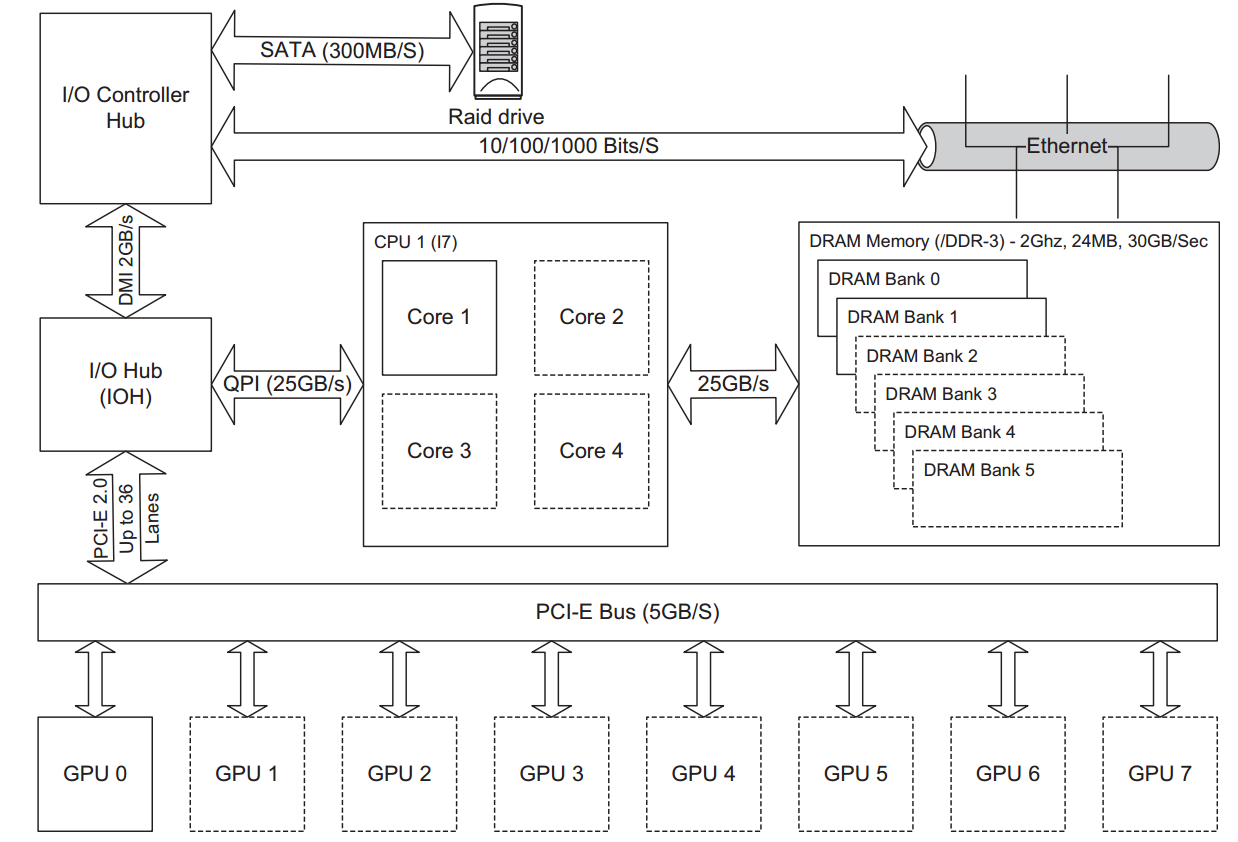
\includegraphics[width=0.7\textwidth]{1_1.PNG}
	\caption{Nehalem/X58 System}
	\label{pl1}
\end{figure}
\begin{figure}[!h]\centering
	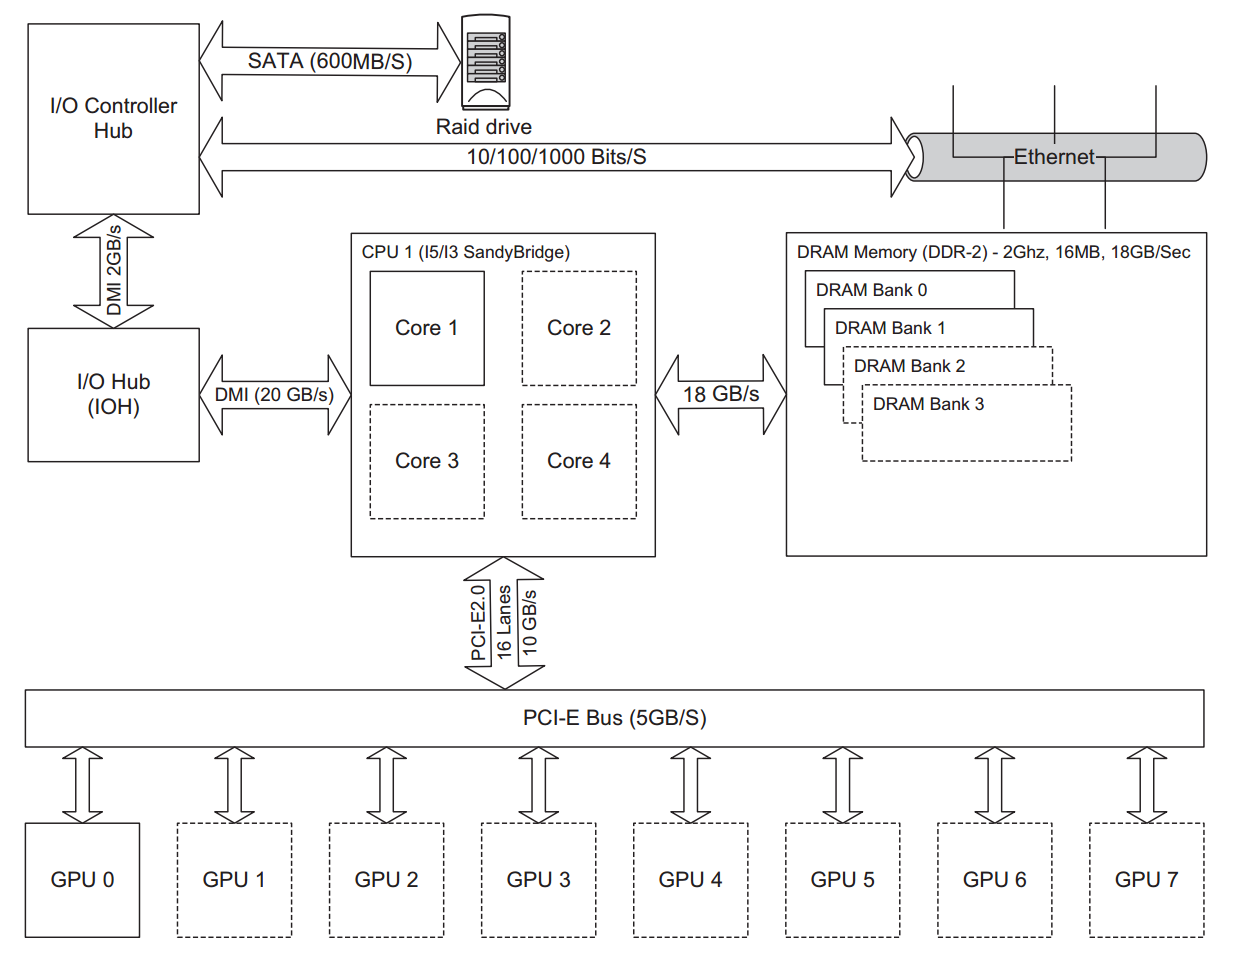
\includegraphics[width=0.7\textwidth]{1_2.PNG}
	\caption{Sandybridge Design}
	\label{pl1}
\end{figure}
\begin{itemize}
	\item What is the difference between peripheral connection in these architectures?

	One of the most noticeable improvements of Sandybridge was the support for the SATA-3 standard, which supports
	600 MB/s transfer rates. This, combined with SSDs, allows for considerable input/output (I/O)
	performance with loading and saving data. While in the Nehalem/X58 architecture peripheral transfer rate is only 300 MB/s. One significant advantage of the AMD chipsets over the Intel ones is the support for up to six SATA
	(Serial ATA) 6 GB/s ports. SATA3 can very
	quickly overload the bandwidth of Southbridge when using multiple SSDs (solid state drives). A PCI-E
	bus solution may be a better one, but it obviously requires additional costs. 
	
	\item Does peripheral connection speed matters? Explain.
	
	 If you consider that the slowest component in any system usually limits the overall throughput, this is something that needs some consideration. For example, SATA3 can very
	 quickly overload the bandwidth of Southbridge when using multiple SSDs (solid state drives). As another fact, If using MPI (Message Passing Interface), which is commonly used in clusters, the latency for this
	 arrangement can be considerable if the Ethernet connections are attached to the Southbridge instead
	 of the PCI-E bus. Consequently, dedicated high-speed interconnects like InfiniBand or 10 Gigabit
	 Ethernet cards are often used on the PCI-E bus.
	 
	\item What kind of port is used to connect to the GPU? What are the attributes of this port?
	
	PCI-E is used. PCI-E (Peripheral Communications Interconnect Express) is an interesting bus as, unlike its
	predecessor, PCI (Peripheral Component Interconnect), it’s based on guaranteed bandwidth. In the
	old PCI system each component could use the full bandwidth of the bus, but only one device at
	a time. Thus, the more cards you added, the less available bandwidth each card would receive. PCI-E
	solved this problem by the introduction of PCI-E lanes. These are high-speed serial links that can be
	combined together to form X1, X2, X4, X8, or X16 links. Most GPUs now use at least the PCI-E
	2.0, X16 specification, as shown in Figure 3.1. With this setup, we have a 5 GB/s full-duplex bus,
	meaning we get the same upload and download speed, at the same time. Thus, we can transfer 5 GB/
	s to the card, while at the same time receiving 5 GB/s from the card. However, this does not mean
	we can transfer 10 GB/s to the card if we’re not receiving any data (i.e., the bandwidth is not
	cumulative).
	
	\item According to the given architectures in figure 1.1 and figure 1.2, how many GPUs can be connected in each system? What about their bandwidth? Explain.
	
	In both cases, 8 GPUs can be connected to the system via PCI-E bus. however, the big downside of socket 1155 Sandybridge design: It supports only 16 PCI-E
	lanes, limiting the PCI-E bandwidth to 16 GB/s theoretical, 10 GB/s actual bandwidth. Thus each GPU is able to use $\frac{10}{8} = 1.25$ GB/s of bandwidth available. On the other hand, the \textit{Nehalem/X58} provides $\frac{16}{8} = 2$ GB/s of bandwidth.
\end{itemize}
\end{document}